% !TEX encoding = UTF-8 Unicode
\documentclass[12pt,twoside]{report}
\usepackage[utf8]{inputenc}
\usepackage[T1]{fontenc}
\usepackage[francais]{babel, varioref}

\usepackage{afterpage}
\usepackage{calc}
\usepackage{color}
\usepackage{fancyhdr}
\usepackage{float}
\usepackage{graphicx}
\usepackage{helvet}
\usepackage{listings}
\usepackage{listingsutf8}
\usepackage{lscape}
\usepackage{textcomp}
\usepackage{xcolor}
\usepackage{xspace}
\usepackage[urlcolor=blue, linkcolor=black,linktoc=all, colorlinks=true]{hyperref}
\usepackage[left=2cm, right=2cm, top=2.1cm, bottom=2.5cm]{geometry}
\usepackage[final]{pdfpages}

\let\iint\undefined
\let\iiint\undefined

\begin{document}
\title{2D matrice pattern search}
\date{March 2018}
\maketitle

\clearpage

\setcounter{tocdepth}{4}
\setcounter{secnumdepth}{4}
\setcounter{page}{1}

\tableofcontents{}

%En cas d'ajout de .tex, copiez-collez cette ligne en modifiant le nom de fichier
% !TEX encoding = UTF-8 Unicode
\chapter{Backlogs}

\section{Project structure - 2h}
Implementation of solution code structure.

\begin{figure}[h]
    \begin{center}
        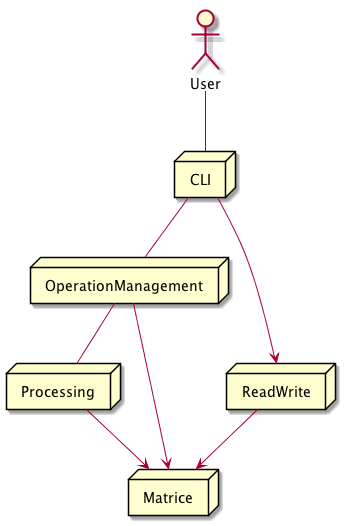
\includegraphics[scale=0.40]{./ressources/graph/deployment.png}
    \end{center}
    \caption{Deployment diagram}
    \label{Solution - Deployment diagram}
\end{figure}
\bigskip


\section{Command line interface - 1/2 day}
It should handle user entry in order to perform search.\\
It should process user entry to extract request information.\\
Assuming that the matrix data contains sensitive information, it should not be stored in plain text:\\
- Command line interface should handle system arguments specifying file path and encryption key.\\
- CLI should work with File processing class in order to work with specified file.\\
\begin{enumerate}
    \item user interface - 30m
    \item user entries processing - 2h30
    \item unit tests - 1h
\end{enumerate}

\section{Matrice structure - 1.5 day}
In order to optimise research, and to be able to perform several research on the same matrice,\\
we should store 2 dimensional matrix of integers from the plain text file into an optimal data structure.\\
Some time should be taken to review the different data structure possible, and responding to search criteria.\\
Algorithm will need to be implemented in order to perform 2D matrix from original file.\\
\begin{enumerate}
    \item Matrice data structure - 1/2d
    \item formating algorithm - 1/2d
    \item unit tests - matrice access, simple research - 1/2d
\end{enumerate}

\section{Operations management - 2 hours}
Handle pattern search request.\\
Manage list of operations to apply on specified 2D matrice.

\section{Search Features - 1.5 day}
There are 3 search functions to implement:
\begin{description}
    \item [search sequence] Find all rows that have a specific sequence of numbers (if that number sequence
appears more than once for that row, you only need to print it once)
    \item [search unordered] Find all rows that contain all of the required numbers (if number repeats, that row must
contain at least that many number)
    \item [search closest match] Find the row that has the closest match to a specific number sequence (just need to
consider the number of matches)
\end{description}
Search features should be of better complexity than O(n) (n is matrix element count).\\

\begin{enumerate}
    \item search management - 2h
    \item search algorithm - 1d
    \item units test - 1/2d
\end{enumerate}

\section{File Processor - 1 day}
User must be able to indicate the matrix data file they will be using through parameters(argc/argv).\\
File processor should be able to read the data from the plain text file into a simple data structure (array).\\
Assuming that the matrix data contains sensitive information, it should not be stored in plain text;\\
File processor should handle an encryption algorithm to hide/access sensitive information.\\
\begin{enumerate}
    \item read/write - 2h
    \item encryption - 1/2d
    \item file processing - 1h
    \item unit tests - 1h
\end{enumerate}

% !TEX encoding = UTF-8 Unicode
\chapter{Planning}

\section{Resumed Backlogs}
\begin{enumerate}
    \item Project structure - 2h
    \item Command line interface - 1/2d
    \item Matrice - 1.5d
    \item Operations management 2h
    \item Search features 1.5d
    \item FileProcessor 1d
\end{enumerate}

\section{Sprints}

Division into sprints of the development cycle.

\subsection{Sprint 1}
Sprint 1 should take 1.5 days.\\
This time will be used to review further the application organisation, and review algorithms to encrypt/unencrypt file.\\
It will contain the initialisation of the application code structure.\\
The implementation of reading and processing method for 2 dimensional matrix of integers representation file.\\
    \begin{itemize}
        \item 1 - Project structure
        \item 6 - File processor
    \end{itemize}

\subsection{Sprint 2}
Sprint 2 should take around 3.5 days.\\
This time will be used to review possibilities between pattern search algorithm, and data structure optimising research.\\
Implementation of an optimised Matrice data structure.\\
Implementation of 3 types research algorithms responding to requested features.\\
Testing of project criteria.
    \begin{itemize}
        \item 3 - Matrice
        \item 5 - Search features
    \end{itemize}

\subsection{Sprint 3}
Sprint 3 should take around 1.5 day.\\
It implies the implementation of the command line interface.\\
The implementation of search operations management used by CLI.\\
Testing and validation of full workflow.
    \begin{itemize}
        \item 2 - Command line interface
        \item 4 - Operations management
        \item Workflow validation
    \end{itemize}

% !TEX encoding = UTF-8 Unicode
\chapter{Sprint 1 - File Processing}

\begin{figure}[h]
    \begin{center}
        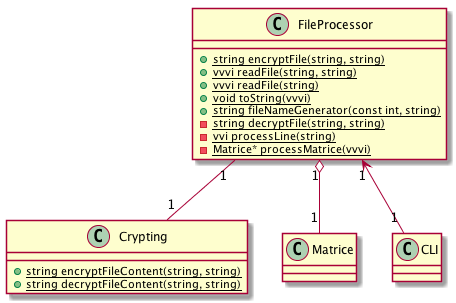
\includegraphics[scale=0.40]{./ressources/graph/FileProcessor.png}
    \end{center}
    \caption{Class diagram}
    \label{Solution - FileProcessing class diagram}
\end{figure}
\bigskip


\section{Matrice format}

In order to have a simple lecture of the plain text file representing a 2 dimensional matrix, with the possibility of
having matrix item of greater dimensions.

\begin{figure}[h]
	\begin{minipage}{0.25\textwidth}
	\flushleft
	Simple 2D Matrix
	\centering
		\begin{verbatim}
		255 255 155
		156 156 157
		255 255 255
		\end{verbatim}
	\end{minipage}
\hfill
\noindent
	\begin{minipage}{0.45\textwidth}
	\flushright
	2D Matrix with multi-dimensional value
		\centering
		\begin{verbatim}
		255,255,255 255,255,255 155,155,155
		156,255,255 156,255,255 157,255,255
		255,255,255 255,255,255 255,255,255
		\end{verbatim}
	\end{minipage}
\label{fig:Plain text matrix format}
\end{figure}

\section{Crypting}

One of the required features was to being handle the case of cipher file.\\
The amount of algorithm and their variants, required us for this project to select a proper and simple crypting method for the:w matrix file the user would used.\\
A decrypting method, but also a crypting method should be developed in order to process properly both plain text and cipher file.

\par
Different crypto libraries have been tested for this features :
\begin{itemize}
	\item openssl
	\item botan
\end{itemize}

\par
First tests with OpenSSL library didn't gave result. The library is low-level, bad-documented and complexify too much the process of encryption and decryption of a file, while for this above feature we were mostly looking for a simple and quick way.

\par
Second test with Botan library gave usefull result. The library is easily accessible (while it still need some cryptographic knowledges to quickly handle availables features).\\
Among the available algorithms (Serpent, AES, Blowfish,etc.) AES-256 has been selected for its broad usage and simplicity.


\section{FileProcessor}

FileProcessor class handle the reading method for both plain text file and cipher file.\\
This class should store the content of user 2D matrix file into a simple data structure (vector), and
give an access the Matrice class which will handle the complexe structure construction algorithm.\\
It also handle the usage of encryption and decryption methods.

\par
FileProcessor class should be the interface between the file selected by the User and the construction of a complexe
matrix data structure.

% !TEX encoding = UTF-8 Unicode
\chapter{Search and Matrix storage}

\par
Search features have to follow several constraints requirements :
\begin{itemize}
	\item Matrice size can be consider of important size, but should fit into RAM at maximum.
	\item Pattern search should be perform on both rows and cols of the matrix.
	\item Search algorithm complexity should not be worse than O(n) with n number of items into the matrix.
	\item No constraints on memory used (max RAM).
\end{itemize}

\section{Search features}

\begin{figure}[h]
    \begin{center}
        \includegraphics[scale=0.40]{./ressources/graph/processing.png}
    \end{center}
    \caption{Search class diagram}
    \label{Solution - Search class diagram}
\end{figure}
\bigskip

\subsection{Matrix items}
Matrix contain only integers, however this value should not be a limit, and we should consider the application of common string search pattern algorithms.\\
The fact that a string search pattern algorithms will mostly look at characteres is not a limit, we consider that such algorithm can be easily modified to handle integer instead of string/characters.\\

A difficulty to handle would be the case of matrix' items of several dimensions (RGBA channel of an image for instance).
\begin{itemize}
	\item A solution would be to simply complexify the comparaison used by search algorithm to work with multiples values. However since the dimensions of matrix' items aren't fixed, this would add complexity to the algorithm.
	\item An other solution would be to process these values through a bijective function, to get a unique values associated to X previous items. This would avoid to complexify the comparaison part of each algorithms.
\end{itemize}


\subsection{Search algorithms}

\par
Last search algorithm complexity requirements impose an important constraints which prevent the usage of pre-process pattern search algorithm. Following algorithms have been studied :
\begin{description}
	\item[Rabin-Karp] : Pre-processing text and pattern with hash function in order to compute associated hash value. Use hash value to reduce comparaison of pattern with string only when hash correspond. In average complexity will be around O(n+m), but worst time performance case will be O(nm) (n as string length, m pattern length).
	\item[Knuth Morris Pratt] : Worst time performance case O(kn) (n as string length, k string search length).
	\item[Finite Automata] : Worst time performance case O(n).
	\item[Boyer Moore] : Worst time performance case O(n + m).
\end{description}

\subsection{Data structure - Suffix tree}

\begin{figure}[h]
    \begin{center}
        \includegraphics[scale=0.40]{./ressources/graph/matrice.png}
    \end{center}
    \caption{Matrix class diagram}
    \label{Solution - Matrice data structure class diagram}
\end{figure}
\bigskip

\par
There is no restriction on the preprocessing of the matrice data. We can consider look at text pre-processing search algorithms.\\
Since several pattern search operations much be perform on a static matrix, suffix tree is a structure which could validate the different constraints of the search features.\\
\begin{itemize}
	\item Constraints are only on search features, so we can consider pre-processing of the text on bigger time performance.
	\item Suffix tree will allow us earch of pattern in O(m) time with m length of the pattern.
	\item Pattern search with mistakes are allowed.
\end{itemize}

\par
In order to handle rows and cols from our matrix, we will have to construct a suffix tree or array tree.\\
Generalised suffix tree : Ukkonen algorithms would allow us to construct a simple suffix tree in O(n).\\
Since we are working with a non-constant "alphabet" (integer values of our matrix), the complexity will be at O(nlogn)
for a simple sentence. We will consider each row and each column of our matrix as a single sentence. By concatening them we will propably lose the linear property of Ukkonen algorithm, however it is a simple way to construct a generalized suffix tree, with time complexity which we can still consider as correct.\\

\par
In our case this data structure would suits perfectly since we have to handle pattern search for a list of rows/cols sequences.

% !TEX encoding = UTF-8 Unicode
\chapter{Sprint 3 - CLI}

\section{Program arguments}
\par
Program is expected 1 to 3 arguments before launching the CLI.
\par
When launching the program the user can give different arguments to the program :
\begin{enumerate}
    \item filePath : simple path to a plain text file path
    \item encrypt filePath password : simple path to a plain text filewhich will be encrypted
    with given password. Output from the CLI will be the path of the cipher file.
    \item cipherFilePath password : path to the cither file, which will be decrypted with the given password.
\end{enumerate}

Based on these different arguments, the main program will handle encryption and decryption
of the file (with FileProcessor class), then send the raw data extracted to the CLI.

\section{CLI}

\begin{figure}[h]
    \begin{center}
        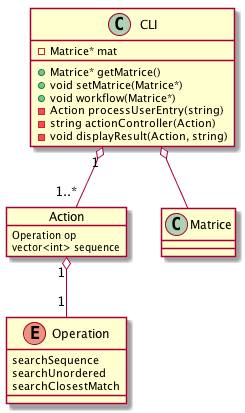
\includegraphics[scale=0.40]{./ressources/graph/CLI.png}
    \end{center}
    \caption{Class diagram}
    \label{Solution - CLI class diagram}
\end{figure}
\bigskip

A simple console log interface (CLI) have been developed in order to enable user to use the pattern research program.\\
Since we don't have to handle a list of operations, the Operation Management class haven't been implemented for simplification of the application.

The CLI is doing the following operations :
\begin{enumerate}
    \item Processing user entry
    \item Calling search operations based on user request and matrice.
    \item Displaying results.
\end{enumerate}


% Liste des figures
\listoffigures

% Bibliographie

\nocite{*}
%\bibliography{tex/biblio}{}
%\bibliographystyle{plain}
%\printbibliography

% Annexes
\clearpage
\appendix
\input{tex/annexes.tex}

\end{document}
